\chapter{Conclusion et perspectives}\label{chap:Conc}%\addcontentsline{toc}{chapter}{\nameref{chap:Conc}}
%\markboth{CONCLUSION}{}
%\mylocaltoc

%\section{Section}

\section{Conclusion générale}

%Cette thèse expérimentale porte sur un réfrigérateur thermoacoustique compact, conçu lors du projet ANR \textsc{Tacot}. Cette machine exploite les interactions entre des ondes sonores de fort niveau et un matériau poreux (appelé "régénérateur") pour générer un flux de chaleur le long de celui-ci. Un volume élémentaire de fluide subit un cycle thermodynamique causé par les oscillations de pression et de position. Cette machine a pour application industrielle prévue la climatisation automobile, et requiert donc une géométrie compacte. La cavité thermoacoustique contenant le noyau est coaxiale, avec face au piston de la source acoustique un guide d'onde 
%
%Au cours de la caractérisation de cette machine, des écarts entre les résultats de mesures et les résultats de la théorie linéaire de Rott ayant servi à sa conception ont été mesurés, tels que des gradients de températures non-linéaires le long de l'axe du régénérateur, ou des non-uniformités de températures sur la section du c\oe{}ur thermoacoustique. Ces dernières sont attribuées à des circulations de fluide dans la machine causées par la convection naturelle, et la vérification de cette hypothèse se fait en réalisant des expériences sous diverses orientations, à différentes amplitudes acoustiques. Le dispositif expérimental existant pour la caractérisation du réfrigérateur est adapté pour répondre aux interrogations formulées. La température est acquise en différents point du régénérateurs grâce à un plan de thermocouple coupant le régénérateur par son centre. Trois palans supportent la machine et permettent de pivoter la machine dans quatre orientations d'intérêt. Quatre orientations sont retenues. La première est celle dans laquelle les expériences de caractérisation de la machine ont été réalisées. Le réfrigérateur est horizontal 
%
%Les résultats expérimentaux montrent que deux zones sont à distinguer. La première est la cavité d'adaptation d'impédance séparant le piston de la source acoustique principale et le noyau thermoacoustique, dont les diamètres sont différents.
La thermoacoustique fait partie d'un domaine interdisciplinaire à l'interface entre l'acoustique, les transferts thermiques et la mécanique des fluides. Elle permet de mettre au point des systèmes de réfrigération au moyen d'ondes acoustiques en exploitant le cycle thermodynamique auquel un volume de fluide est soumis au passage d'une onde acoustique. En introduction, les principes de bases de la réfrigération thermoacoustique issus de la théorie linéaire classique développée par Rott ont été rappelés succintement, ainsi que les limites de ce modèle qui ne tient pas compte de certains effets tels que la génération d'harmoniques dûe à la propagation non-linéaires à forte amplitude, l'apparition d'écoulements tourbillonaires, l'influence des pertes de charges, le vent acoustique ou la convection naturelle. Des écarts entre les résultats du modèle de Rott et des résultats expérimentaux obtenus lors de la caractérisation du réfrigérateur \textsc{Tacot} au cours du projet ANR éponyme sont présentés, et mettent en évidence la présence d'effets supplémentaires qui se superposent à l'effet thermoacoustique attribués à la présence d'écoulements liés à la convection naturelle. Cet effet est assez peu étudié dans le cas des réfrigérateurs thermoacoustiques, ce qui motive ce travail de thèse expérimental qui porte sur les mesures de distributions complexes de température au c\oe{}ur de la machine thermoacoustique.\medskip
%L'auteur commence par présenter les concepts généraux de la thermoacoustique, les équations fondamentales de l'acoustique en fluides dissipatifs, et les fonctions visco-thermiques caractérisant les milieux tortueux. Il présente également des outils électroacoustiques (modèles aux constantes localisées, circuits électriques équivalents, matrices de transfert) utilisés pour modéliser les systèmes thermoacoustiques.\medskip

L'impact de la convection naturelle sur le fonctionnement de la machine est analysé en étudiant les distributions de température au sein du noyau thermoacoustique et à son voisinage, et ses performances. Après la présentation de la géométrie de la machine coaxiale, compacte et à deux sources acoustiques, et conçue pour répondre aux besoins du projet ANR \textsc{Tacot} que sont la compacité et le ciblage du déphasage optimal au sein du régénérateur, l'instrumentation est décrite. Celle-ci reprend le système d'acquisition existant préalablement à cette thèse et est adaptée pour obtenir le plus d'information possibles sur la distribution complexe des températures autour du noyau, ce qui se fait au moyen d'un plan de thermocouples divisant en deux le régénérateur cylindrique le long de son axe. Les données de températures sont acquises et regroupées dans deux zones d'intérêt : la première est le noyau thermoacoustique de la machine, et la seconde est la cavité dont la fonction est d'adapter l'impédance acoustique entre la source et le noyau. L'étude de la convection n'est pas évidente dans ces zones du fait de la porosité du régénérateur d'une part, et de la forme conique de la cavité d'adaptation d'impédance d'autre part. Le reste de l'instrumentation adaptée du système existant permet également de mesurer les pressions acoustiques, les accélérations des sources acoustiques, ainsi que la température d'eau dans l'échangeur de chaleur ambiant.\medskip

L'étude de la convection naturelle requiert de changer l'orientation du réfrigérateur par rapport à la direction de la gravité. Quatre orientations sont choisies pour leur caractère académique, et peuvent être classées en deux catégories. La première comporte deux orientations où l'axe du réfrigérateur est horizontal, avec les thermocouples disposés sur un plan vertical, ou horizontal. La seconde catégorie comprend deux orientations où le réfrigérateur est vertical, avec dans un cas le côté froid du noyau placé en bas de celui-ci et dans l'autre, au dessus. Le dispositif expérimental est donc adapté à cette étude pour permettre ces rotations, en utilisant des palans pour suspendre la machine lourdement instrumentée et dont la masse est élevée. Un protocole est développé pour assurer des résultats d'expériences clairs. Pour cela, plusieurs étapes préliminaires sont suivies, en procédant en premier lieu à l'acquisition des conditions initiales de toutes les variables mesurées pour les prendre en compte dans l'analyse, et en fixant le temps d'acquisition à \qty{1}{\hour} pour garantir l'observation du régime transitoire entier et de tout évènement qui pourrait s'y produire. Différents types d'expériences sont réalisés avec et sans champ acoustique, afin de dissocier les effets thermiques seuls de ceux de la thermoacoustique.\medskip


Une approche théorique de la convection naturelle dans les différentes zones de la machine est proposée. Tout d'abord, des ordres de grandeur du nombre de Rayleigh sont calculés pour caractériser la propension du fluide de travail à se mettre en mouvement suite à l'apparition des gradients de températures provoqués par l'effet thermoacoustique. Cette étude est menée dans les cas de la cavité d'adaptation d'impédance remplie du mélange de gaz et du régénérateur poreux. Cette analyse préliminaire permet de calculer des ordres de grandeurs des vitesses de circulation du fluide. Il ressort de cette étude que des cellules de convection peuvent apparaître au sein de la cavité d'adaptation d'impédance, mais pas dans le régénérateur. Une simulation numérique par éléments finis d'un problème thermique analogue à la machine thermoacoustique est réalisée à l'aide du logiciel \textsc{Comsol}, pour étudier plus avant la circulation de fluide dans la cavité d'adaptation d'impédance mise en évidence par l'étude du nombre de Rayleigh. Deux configurations sont présentées : l'une comporte la cavité d'adaptation d'impédance seule dans des orientations où le gradient de température fixé par les conditions aux frontières est vertical ; l'autre utilise cette même cavité cette fois-ci couplée à un modèle simplifié du noyau thermoacoustique, dans les quatre orientations étudiées. Conformément au calcul du nombre de Rayleigh appliqué aux milieux poreux qui ne prédit pas la présence d'écoulements de convection dans le régénérateur, celui-ci est simulé par un solide homogène. L'empilement de tissus métalliques dans le régénérateur est pris en compte dans ce modèle par l'utilisation d'une matrice de conductivité thermique traduisant la dégradation de celle-ci et l'anisotropie de ce matériau. Ces études montrent des résultats différents de ce que prédit l'étude du nombre de Rayleigh, notamment que la géométrie conique de la cavité provoque l'apparition de cellules de convection dans des configurations \textit{a priori} stables dans certaines orientations. Ce modèle rudimentaire est complété par un modèle du régime transitoire qui simule le flux de chaleur généré par l'effet thermoacoustique, le flux de conduction thermique axial et transversal, l'échauffement visqueux et les pertes aux frontières du noyau. Ce modèle à deux dimensions spatiales contient des termes sources, et le problème thermique est résolu à l'aide de la méthode des transformations intégrales. Cependant, les paramètres du modèle doivent encore être ajustés au moment de la rédaction de ce manuscrit.\medskip

Des expériences sont menées à différentes amplitudes acoustiques, avec différentes charges thermiques imposées par les échangeurs de chaleur, et pour les orientations choisies.  Les distributions de températures sont tout d'abord analysées en séparant les résultats d'expériences sans et avec un champ acoustique, et marquent la présence de cellules de convection naturelle dans la cavité d'adaptation d'impédance, et l'absence de circulation de fluide par convection naturelle dans le régénérateur. Dans les configurations où le réfrigérateur est placé à l'horizontale, la convection naturelle fait apparaître des gradients de température sur la direction transverse verticale et romp l'axisymétrie du système. Dans celle où il est vertical, les températures mesurées du côté froid du noyau sont plus élevées dans une orientation que dans l'autre, ce qui montre la présence d'un flux montant d'une zone plus chaude dans le cas où celle-ci se trouve en dessous. Enfin, l'augmentation de l'amplitude accroit les différences de températures susceptibles de provoquer la mise en mouvement du fluide, mais fait apparaître dans le même temps d'autres effets liés aux hautes amplitudes acoustiques mentionnés plus haut. Les effets liés à la convection naturelle sont ainsi de moins en moins visibles. Un point de vue énergétique de la machine enfin adopté en observant les températures moyennées des côtés froid et ambiant du noyau, les flux de chaleur apportés et extraits par les échangeurs, et les coefficients de performances rapportés à Carnot. Les résultats laissent penser que l'orientation a assez peu d'impact sur les flux de chaleurs transportés. En revanche, les températures sont impactées par la gravité, et avec elles, le coefficient de performances qui en dépend.
%
%démontrent l'impact significatif de la convection naturelle sur les performances du réfrigérateur thermoacoustique. Cet impact varie selon l'orientation du dispositif par rapport à la gravité. Les résultats montrent que :
%
%    Le coefficient de performance (COP) du réfrigérateur est fortement affecté par l'orientation
%
%    Les températures atteintes dans le régénérateur dépendent de la présence ou non de convection
%
%    La distribution des températures dans la cavité d'adaptation d'impédance révèle la présence de cellules convectives qui influencent le transfert thermique
%
%Les mesures réalisées avec et sans champ acoustique permettent de distinguer les effets purement convectifs des effets thermoacoustiques, et mettent en évidence leur interaction dans le fonctionnement global du système.
%Conclusion et perspectives
%
%Cette étude expérimentale approfondie démontre l'importance de prendre en compte les phénomènes de convection naturelle dans la conception et l'optimisation des réfrigérateurs thermoacoustiques. L'auteur propose plusieurs perspectives pour des travaux futurs :
%
%    Des études avancées de la convection dans la cavité conique
%
%    Des analyses plus détaillées de la conduction dans le noyau thermoacoustique
%
%    Des améliorations électroacoustiques, notamment par le contrôle actif et le remplacement des sources acoustiques
%
%    Des simulations par éléments finis plus sophistiquées avec une géométrie plus précise, des conditions aux frontières adaptées et des interfaces physiques améliorées
%
%Ce travail contribue significativement à la compréhension des phénomènes thermiques dans les systèmes thermoacoustiques compacts et ouvre la voie à l'optimisation de ces dispositifs pour des applications pratiques.



\section{Perspectives}



\subsection{Expérimentations supplémentaires}

\subsubsection{\'Etudes avancées de la convection dans la cavité conique}
La convection dans la cavité conique a été étudiée expérimentalement dans le chapitre~\ref{chap:EtudeExpe}. Cependant, l'instrumentation dans cette cavité ne comprend que quatre thermocouples, et une étude plus avancée, notamment des champs de vitesse dans cette cavité, serait intéressante pour évaluer les phénomènes de convection mis en évidence. En particulier, les conditions aux frontières sont très importantes dans la compréhension des mouvement de fluide dans la cavité~\cite{mergui_convection_1996}, et une version académique de celle-ci pourrait apporter beaucoup d'informations sur le comportement du fluide près des frontières.

\subsubsection{\'Etudes avancées de la conduction dans le noyau}
\paragraph{\'Etude de la conduction par les parois du noyau thermoacoustique}
La conduction par les parois du noyau thermoacoustique est un facteur très important à prendre en compte. En effet, lorsque le réfrigérateur fonctionne et qu'un gradient de température s'établit le long du régénérateur, un flux de chaleur \og retour \fg{} de conduction apparaît dans le sens opposé au flux de chaleur thermoacoustique. Comme le matériau poreux qui compose le régénérateur, il n'est pas nécessaire que les parois soit conductrice de chaleur. Pour une prochaine étape d'étude de la distribution de température dans le noyau thermoacoustique, l'enveloppe qui contient les disques de tissu métallique et qui est initialement usinée dans un cylindre d'acier inoxydable est remplacée par une pièce similaire imprimée en plastique. L'ABS est choisi pour la fabrication de ce nouveau contenant plutôt que le PLA, car ce dernier peut se ramollir sous l'action des températures atteintes dans certaines expériences, c'est-à-dire autour de \qtyrange{50}{60}{\degreeCelsius}. Dans le cas de l'ABS, cette température limite d'utilisation est élevée à \qty{100}{\degreeCelsius}.
\medskip

L'enveloppe imprimée en 3D, qu'il conviendrait de mettre en place pour contenir les disques de tissus métalliques du noyau, est présentée sur la figure~\ref{fig:CanisterPlastique}.

\begin{figure}[!ht]
	\centering
	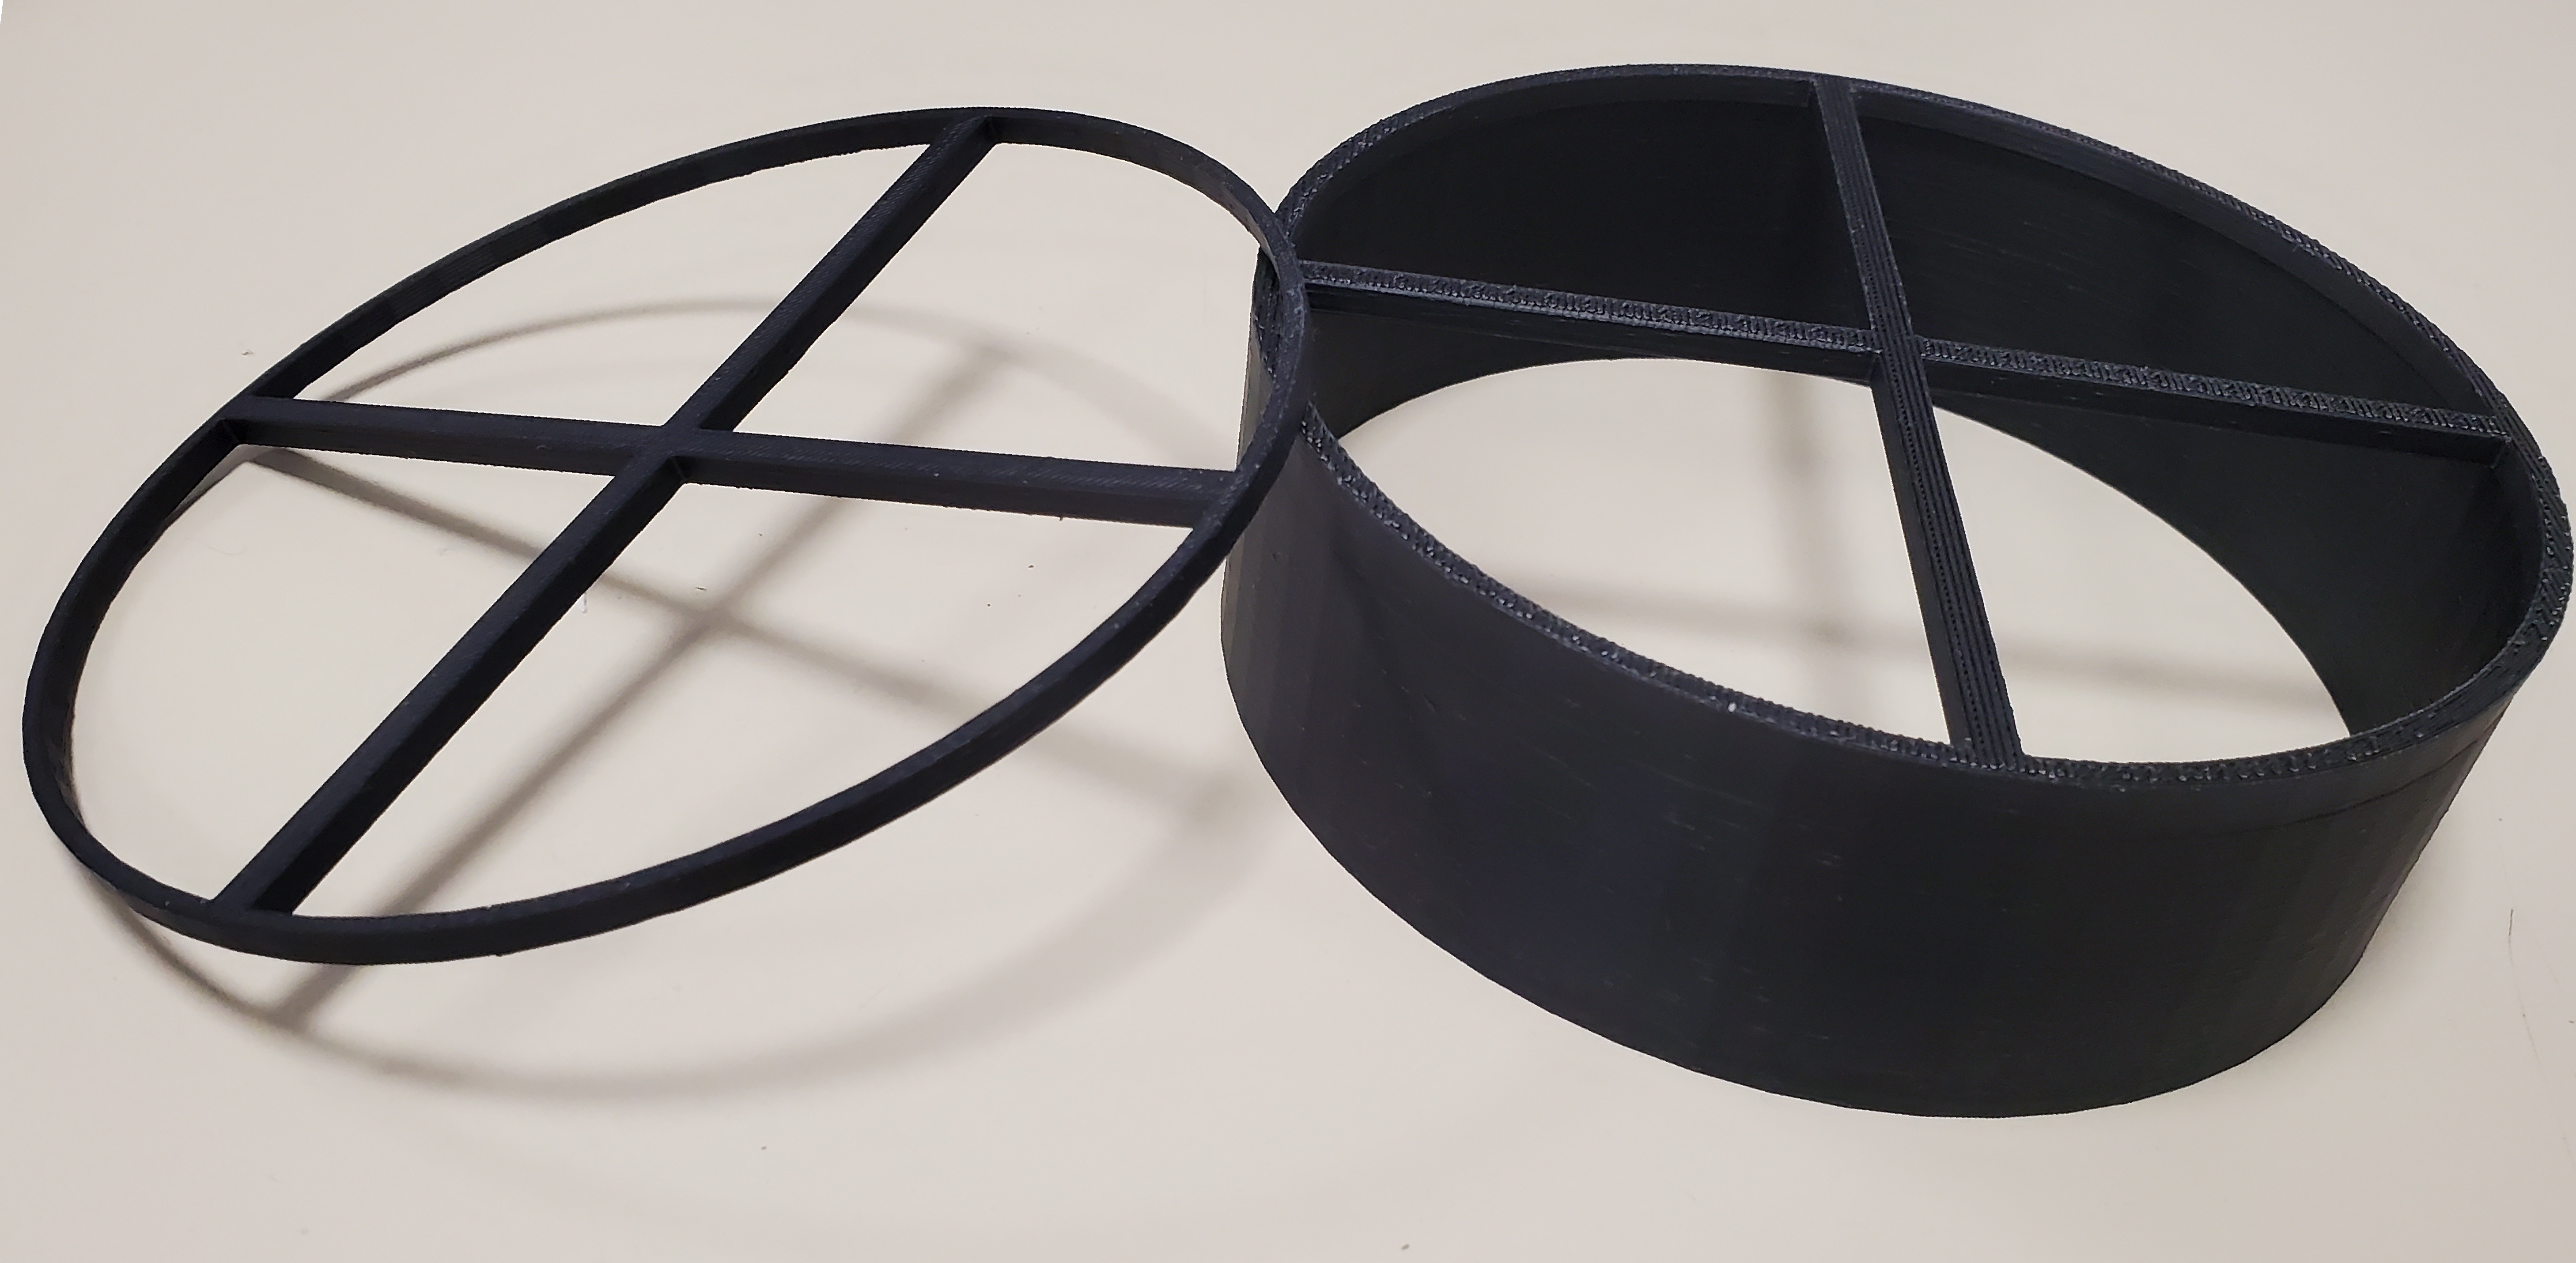
\includegraphics[width=.7\textwidth]{../fig/fig_CanisterPlastique/fig_CanisterPlastique.pdf}
	\caption{Enveloppe contenant les disques de tissus métalliques du noyau thermoacoustique, imprimé en 3D en ABS.}
	\label{fig:CanisterPlastique}
\end{figure}

\paragraph{Conductivité de l'empilement de disques de tissus métalliques}
La comparaison entre les simulation numériques et les expériences (voir les figures~\ref{fig:Comsol_CHXout_H1H2_Low} et \ref{fig:Comsol_CHXout_V1V2_Low}) montre que l'estimation de la conductivité d'après la définition de $\mathbf k_{\sf tissus}$ dans l'équation~\eqref{eq:ConductiviteTensiorielle} est incorrecte. En effet, les termes extradiagonaux sont certainement non-nuls. Un travail avancé sur l'estimation de cette conductivité doit être fait, pour déterminer les coefficients d'une nouvelle matrice $\mathbf k_{\sf tissus}$ de la forme

\begin{equation}
	\mathbf k_{\sf tissus} = \begin{bmatrix}
	k_{xx} & k_{xy} & k_{xz} \\
	k_{yx} & k_{yy} & k_{yz} \\
	k_{zx} & k_{zy} & k_{zz} 
	\end{bmatrix}
	\label{eq:ConductiviteTensorielle_FullAnisot}
\end{equation}



\subsubsection{\'Electroacoustique}

Dans l'optique de poursuivre l'amélioration de cette pompe à chaleur thermoacoustique, l'aspect des sources acoustiques reste à considérer.

\paragraph{Contrôle actif}
Le champ acoustique doit être contrôlé avec précision, en particulier l'impédance acoustique et son déphasage au sein du matériau poreux. Dans l'état actuel de la machine, les sources acoustiques sont contrôlées manuellement, et le déphasage inter-sources acoustiques est réglé sur le générateur de signaux. Une étude de l'asservissement de la source secondaire au moyen d'un dispositif de traitement du signal en temps réel tel que le \textit{digital signal processor} ADAU1701 de SigmaDSP (figure~\ref{fig:ActiveControl_ADAU1701}) ou un Teensy~4.1 (figure~\ref{fig:ActiveControl_Teensy41}) permettrait d'atteindre le champ acoustique optimal.



\begin{figure}[!ht]
    \centering
	\begin{subfigure}{.47\textwidth}
		\centering
		\external{fig_ActiveControl_ADAU1701}
		\tikz{\draw(0,0) node{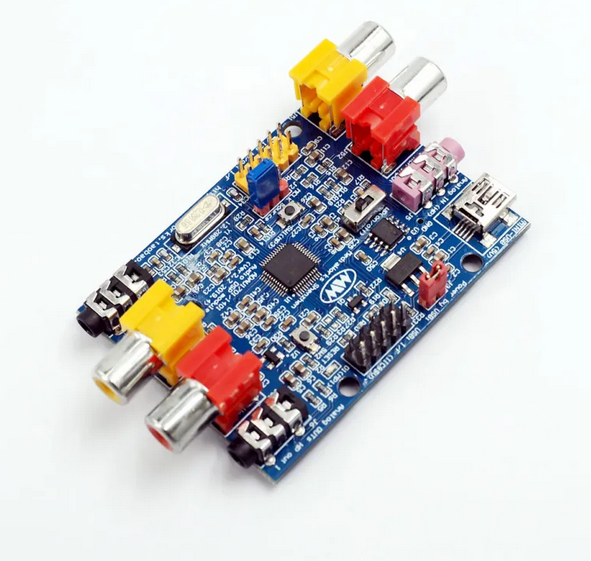
\includegraphics[height=5cm]{../fig/fig_ActiveControl/ADAU1701}};}
		\caption{}
		\label{fig:ActiveControl_ADAU1701}
	\end{subfigure}		
	\begin{subfigure}{.47\textwidth}
		\centering
		\external{fig_ActiveControl_Teensy41}
		\tikz{\draw(0,0) node{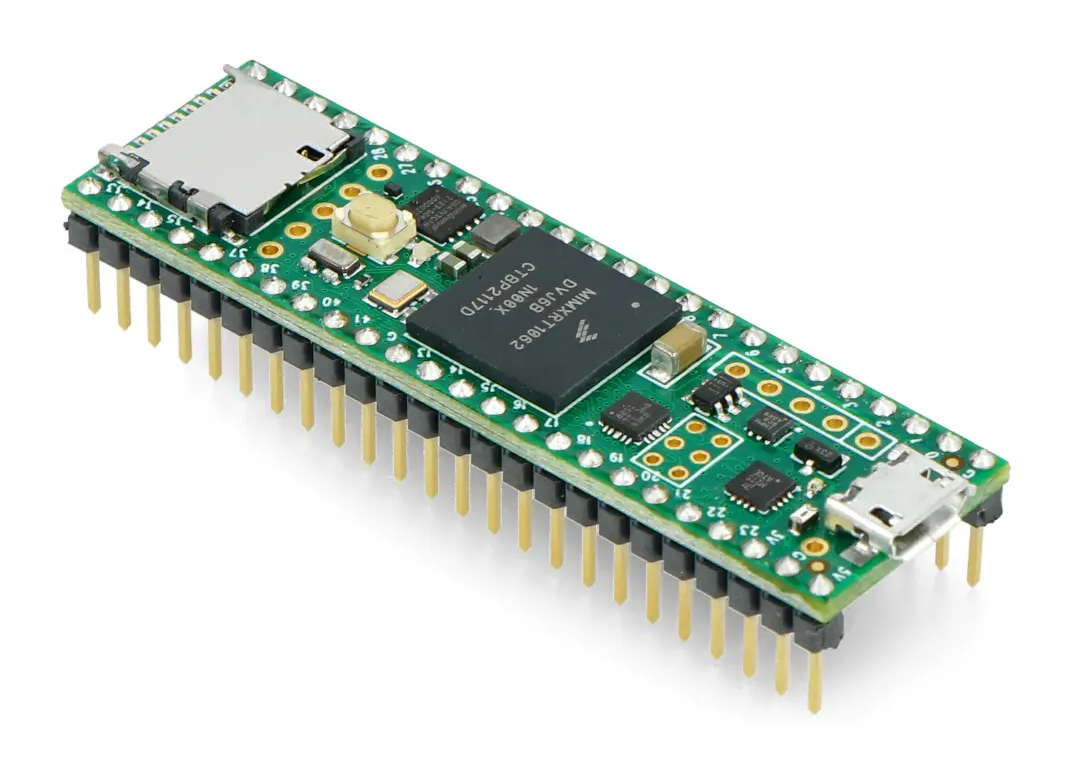
\includegraphics[height=5cm]{../fig/fig_ActiveControl/Teensy41}};}
		\caption{}
		\label{fig:ActiveControl_Teensy41}
	\end{subfigure}	    
    \caption{Dispositif de traitement du signal numérique en temps réel. \subref{fig:ActiveControl_ADAU1701} SigmaDSP ADAU1701 et \subref{fig:ActiveControl_Teensy41} Teensy 4.1}
    \label{fig:ActiveControl}
\end{figure}

Ces cartes sont toutefois sources de retards : les différents calculs réalisés par le processeur, les filtres, les conversions analogique-numérique et numérique-analogique prennent du temps, mais il est possible d'atteindre des retards faibles de l'ordre de \qty{80}{\micro\second}, ce qui correspond à un déphasage de \ang{1.35} à la fréquence de fonctionnement du \textsc{Tacot}, \qty{47}{\hertz}. Cette faible valeur rend possible leur utilisation pour un contrôle du champ acoustique dans la cavité thermoacoustique.

\paragraph{Remplacement des sources acoustiques}
\subparagraph{Source principale}
La source acoustique principale est un moteur linéaire. Ce type de source est à la fois onéreux et difficile à se procurer, c'est pourquoi il peut être intéressant d'étudier l'impact sur les performances d'une source alternative. Diverses simulations à l'aide de \textsc{DeltaEC} en utilisant des haut-parleurs du commerce pourrait permettre de faire évoluer la machine vers un système modulaire. En l'occurrence, le haut-parleur du commerce Ciare CSW7012EVO (figure~\ref{fig:CiareCSW7012EVO}) semble prometteur au vu du déplacement du piston et du facteur de force $B\ell$.

\begin{figure}[!ht]
\centering
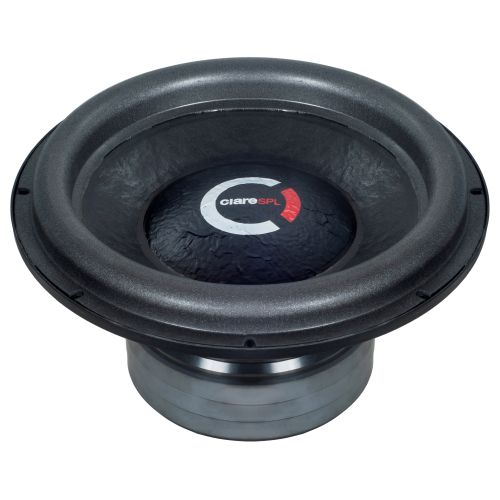
\includegraphics[height=5cm]{../fig/fig_CiareCSW7012EVO/CSW7012EVO}
\caption{Ciare CSW7012EVO}
\label{fig:CiareCSW7012EVO}
\end{figure} 

\subparagraph{Source secondaire}
Le rôle de la source acoustique secondaire est multiple, mais les performances de la machine pourraient être grandement améliorées en utilisant un haut-parleur plus puissant. Une idée serait de concevoir une source acoustique avec un aimant dont le champ magnétique est plus intense, et d'utiliser à la place du cône un piston en nid d'abeille, afin de réduire ses dimensions et ainsi, pouvoir augmenter son déplacement sans heurter l'échangeur ambiant qui se trouve juste en face.

\subsection{Simulations par éléments finis avancées}
\subsubsection{Géométrie}
Les simulations présentées dans la section~\ref{chap:FEM} ne prennent en compte que la cavité d'adaptation d'impédance, le régénérateur solide et l'enceinte qui le contient. Ce choix permet de limiter les couplages thermiques et les difficultés de calcul qui les accompagnent, et fait suite à une hypothèse formulée sur la prédominance de la conduction thermique dans le régénérateur sur les autres effets. Cela se manifeste par l'usage d'une condition adiabatique pour la paroi extérieure de l'enceinte. 

Cependant, la présence de la boucle de rétroaction introduit un couplage entre cette paroi extérieure, et l'extérieur de la machine. Pour ajouter cette condition aux frontières du noyau, le domaine correspondant au fluide devra étendu, pour englober la boucle de rétroaction, ainsi que l'espace situé entre le côté ambiant du noyau et la source acoustique secondaire. La géométrie de ce modèle avancé avec les conditions aux frontières correspondantes est dessinée sur la figure~\ref{fig:Geometrie_FeedbackLoop}.

\begin{figure}[!ht]
	\centering
	\external{fig_Geometrie_FeedbackLoop}
%	\externalremake
	\begin{tikzpicture}[scale=1/3]
	\def\rCHX{7cm};
	\def\lCHX{.7cm};
	\def\rREG{7.4cm};
	\def\lREG{3.9cm};
	\def\rCAN{15.6/2*1cm};
	\def\lCAN{\lREG};
	\def\rAHX{5.5cm};
	\def\lAHX{2.3cm};
	\def\rRIX{5.4cm};
	\def\rCONE{8.2cm};
	\def\lTA{\lAHX+\lREG+\lCHX};
	
	
	\draw[dashed] (0,-\rREG) rectangle (\lTA,\rREG) (0,-\rCAN) rectangle (\lTA,\rCAN);
	\draw[MatlabYellow] (0,-\rCONE) -- (-3*\lAHX,-\rRIX) -- ++(0,2*\rRIX) -- (0,\rCONE) -- (\lTA+1cm,\rCONE) -- ++(0,-2*\rCONE) -- cycle;
	
	\draw[MatlabOrange, line width=1mm] (\lTA,-\rCAN) -- ++(0,2*\rCAN) node[above right, rotate=45]{$Q=\qty{3}{\watt}$};
	\draw[MatlabBlue, line width=1mm] (0,-\rCAN) -- ++(0,2*\rCAN) node[above right, rotate=45]{$Q=\qty{-3}{\watt}$};
	\draw[MatlabYellow, line width=1mm] (-3*\lAHX,-\rRIX) -- ++(0,2*\rRIX) node[above right, rotate=45]{$\mathbf n \cdot \mathbf Q=0$} (\lTA+1cm,-\rCONE) -- ++(0,2*\rCONE);
\end{tikzpicture}
	\caption{Géométrie prenant en compte la boucle de rétroaction pour le modèle \textsc{Comsol}\textss\textregistered}
	\label{fig:Geometrie_FeedbackLoop}
\end{figure}

\subsubsection{Conditions aux frontières adaptées}
Les conditions aux frontières doivent être modifiées pour représenter le modèle. Les parois régénérateur-enceinte, et enceinte-boucle de rétroaction sont modélisées par une continuité des flux de chaleur et des températures, la paroi correspondant à l'échangeur ambiant est considérée comme une source de chaleur apportée par l'effet thermoacoustique, et les parois représentant les sources acoustiques sont traitées comme des parois adiabatiques.

\subsubsection{Interface physique}
Enfin, dans ce modèle, il serait également très intéressant de considérer les effets de la porosité sur le comportement du régénérateur, en particulier sur l'existence de circulations causées par la convection naturelle à l'intérieur du noyau. Cela se fait par l'interface \texttt{Brinkman equations (br)}, qui n'avait pas été incluse dans le modèle du paragraphe~\ref{chap:FEM} qui constituait une première approche.

\subsection{Modèle transitoire}
Les résultats numériques obtenus par simulation du régime transitoire sont présentés pour une seule orientation `\texttt{H2}'. Les amplitudes de températures sont incorrectes, le plus probablement à cause d'un mauvais ajustement des coefficients d'échanges convectifs $h$. Il est nécessaire d'obtenir les coefficients correspondants à chaque configuration (orientation, amplitude acoustique) pour simuler correctement le \textsc{Tacot}.



